\section{Optimization Algorithms}

\subsection{Active Set Methods}

Used when you have a good heuristic for active set.

\begin{algorithmic}[1]
    \STATE Find a feasible starting point
    \WHILE {not ``optimal enough''}
      \STATE Solve the equality problem defined by the active set (approximately).
      \STATE Compute the Lagrange multipliers of the active set.
      \STATE Remove a subset of the constraints with negative Lagrange multipliers.
      \STATE Search for infeasible constraints.
    \ENDWHILE
\end{algorithmic}

\subsection{Barrier / Interior Point}

\begin{itemize}
    \item Replace inequalities with barrier function in objective:
    \begin{equation}
        \begin{array}{c}
            \min\text{\,\,}f\left( x \right)\\
            \text{s.t.\,\,}c\left( x \right) \le 0\\
        \end{array}\Rightarrow \min_xf\left( x \right) -\sum{\frac{1}{\rho _i}\log \left( -c_i\left( x \right) \right)}
    \end{equation}
    \begin{figure}[H]
        \centering
        
\includegraphics[scale=.75]{./tex/ch5/1.pdf}
        \caption{Barrier Function: $-\log(-x)$.}
    \end{figure}
    \item The idea is that the barrier function blows up to infinity at the constraint boundary and keeps it away from going across the boundary so that's why they're called interior points because they always stay inside the feasible set or interior of the constraints. 
    \item The barrier function does not have to be $\log$, it just has to blow up at the boundary.
    \item It is the gold standard for small to medium \textcolor{red}{convex} problems.
\end{itemize}

\subsection{Penalty}

\begin{itemize}
    \item \textcolor{red}{This is a dumb method, never use it.} But it leads to augmented Lagrangian method.
    \item Replace constraints with penalty term that penalizes violations:
    \begin{equation}
        \begin{array}{c}
            \min\text{\,\,}f\left( x \right)\\
            \text{s.t.\,\,}c\left( x \right) \le 0\\
        \end{array}\Rightarrow \min_xf\left( x \right) +\frac{\rho}{2}\left[ \max \left( 0,c\left( x \right) \right) \right] ^2
    \end{equation}
    \item The key difference between penalty methods and barrier methods is that barrier methods blow up at the boundary and you never cross the boundary, while penalty methods don't do anything in the interior until you cross the boundary so they're always basically trying to pull you back and you're kind of always violating constraints a little bit right. You're always outside the constraint boundary and the penalty is pulling you back, while barrier functions push on you from the other side and keep you from ever crossing the boundary. So that's like kind of a key qualitative difference and that's why the barriers are called interior point for that reason. You might hear people call these penalty methods ``exterior'' penalties because they only penalize you once they're outside the constraint.
    \item Easy to implement, but they don't work well in practice because it turns out in order to actually get that constraint to be satisfied, $\rho$ penalty weight goes up to infinity and you can never do that obviously and well before that you end up with \textbf{numerical ill conditioning} kind of floating point badness (\textbf{low accuracy}).
\end{itemize}

\subsection{Augmented Lagrangian}
\begin{itemize}
    \item Add Lagrange multiplier estimate to penalty method:
    \begin{equation}
        \begin{array}{c}
            \min\text{\,\,}f\left( x \right)\\
            \text{s.t.\,\,}c\left( x \right) \le 0\\
        \end{array}\Rightarrow L_{\rho}\left( x,\tilde{\lambda} \right) =\min_xf\left( x \right) +\tilde{\lambda}^T\max\left( 0,c\left( x \right) \right) +\frac{\rho}{2}\left[ \max \left( 0,c\left( x \right) \right) \right] ^2
    \end{equation}
    There are two ways to look at this, you can either look at it as penalty plus a Lagrangian multiplier estimate term or you can look at it as the original lagrangian plus the penalty term. Note here we're only minimizing with respect to $x$, we're not solving the joint $(x, \lambda)$ problem with the KKT system like we were before with the equality constraint, we're only solving a problem in $x$ while we hold $\lambda$ fixed.
    \item Update $\tilde{\lambda}$ by ``offloading'' penalty term into $\tilde{\lambda}$ at each iteration (only when the constraint is violated, a.k.a active constraints):
    \begin{equation}
        \begin{aligned}
            \frac{\partial f}{\partial x}+\tilde{\lambda}^T\frac{\partial c}{\partial x}+\rho c\left( x \right) ^T\frac{\partial c}{\partial x}=&\frac{\partial f}{\partial x}+\left( \tilde{\lambda}+\rho c\left( x \right) \right) ^T\frac{\partial c}{\partial x}\\
            \tilde{\lambda}\gets& \tilde{\lambda}+\rho c\left( x \right)\\
        \end{aligned}
    \end{equation}
    The key insight is that term $\left( \tilde{\lambda}+\rho c\left( x \right) \right)$ is acting just like a Lagrangian multiplier term, it's pushing in the same direction as the Lagrangian multiplier, it's pushing up against the constraint because $\rho$ also pushes against constraints. The intuition is if there's some penalties in here it means one of them is not big enough so just take this entire term. It effectively updates a $\lambda$ estimate from the penalty.
    \item Repeat until convergence:
    \begin{enumerate}
        \item $\min_x L_\rho(x,\tilde{\lambda})$
        \item $\tilde{\lambda}\gets \max(0,\tilde{\lambda}+\rho c\left( x \right))$ (Clamping to guarantee $\tilde{\lambda}\ge0$)
        \item $\rho\gets\alpha\rho$ (Typically, $\alpha\approx10$, when $\rho$ is big enough, stop this operation)
    \end{enumerate}
    \item Fixes ill-conditioning of penalty method.
    \item Converges with finite $\rho$, while pure penalty method only satisfies $c(x)$ exactly when $\rho\to\infty$.
    \item Works well on non-convex problems. (barrier works only for convex)
    \item $\rho\text{(sublinear)} \& \lambda\text{(linear)} \to \text{superlinear}$
\end{itemize}

\subsection{Quadratic Program}
\begin{equation}
    \begin{aligned}
        \min_x\frac{1}{2}x^TQx+&q^Tx,Q\succ 0\\
        \text{s.t.}\ Ax\le& b\\
        Cx=&d\\
    \end{aligned}
\end{equation}
\begin{itemize}
    \item Super useful in control.
    \item Can be solved very fast ($\sim$kHz).
\end{itemize}
\subsection{Example}
\begin{equation}
    \begin{aligned}
        \min_x f(x) =& 0.5  \left(x-\begin{bmatrix}
            1\\0
        \end{bmatrix}\right)^T\begin{bmatrix}
            0.5&0\\0&1
        \end{bmatrix}\left(x-\begin{bmatrix}
            1\\0
        \end{bmatrix}\right) \\
    \text{s.t.}& \qquad x[0] - x[1] < -1
    \end{aligned} 
\end{equation}
Try with penalty, full Augmented Lagrangian, or just $\lambda$ update.

\subsection{Regularization and Duality}
\begin{equation}
    \begin{aligned}
        \min_x f(x) \\
        \text{s.t.} \qquad c(x) = 0
    \end{aligned}
\end{equation}

\begin{itemize}
    \item Remember we did the whole KKT conditions, optimality conditions and lagrangian multiplier story, we're now going to get there by a different path.
    \item We might like to turn this into a weird brick wall penalty:
    \begin{equation}
        \min_xf\left( x \right) +p_{\infty}\left( c\left( x \right) \right) ,\qquad p_{\infty}\left( x \right) =\left\{ \begin{array}{l}
            0,x=0\\
            +\infty ,x\ne 0\\
        \end{array} \right. 
    \end{equation}
    \item Obviously we aren't going to implement an algorithm based on this, but it leads to some interesting stuff.
    \item Practically terrible, but we can get the same effect by solving:
    \begin{equation}
        \min_x\max_{\lambda}f\left( x \right) +\lambda ^Tc\left( x \right) 
    \end{equation}
    \item Whenever $c(x)\ne0$, inner problem blows up.
    \item Similar for inequalities:
    \begin{equation}
        \begin{array}{c}
            \left. \begin{array}{r}
            \min_{\lambda}f\left( x \right)\\
            s.t.\,\,c\left( x \right) \le 0\\
        \end{array} \right\} \rightarrow \min_xf\left( x \right) +p_{\infty}^{+}\left( c\left( x \right) \right) ,\qquad p_{\infty}^{+}\left( x \right) =\left\{ \begin{array}{l}
            0,x\le 0\\
            +\infty ,x>0\\
        \end{array} \right.\\
            \Rightarrow \min _x\max _{\lambda \ge 0}f\left( x \right) +\lambda ^Tc\left( x \right)\\
        \end{array}
    \end{equation}
    \item This min-max problem is actually what we're solving when we solve the KKT system for both $x$ and $\lambda$ jointly at the same time. This is ``duality'' called the Lagrangian dual. 
    \item Interpretation: KKT conditions define a saddle point in $(x,\lambda)$.
    \item KKT system should have $\text{dim}(x)$ positive eigen values and $\text{dim}(\lambda)$ negative eigen valves at an optimum. Called ``quasi-definite'', the KKT system Eq. \eqref{equ:kkt-system} should be:
    \begin{equation}
        \left[ \begin{matrix}
            H+\beta I&		c^T\\
            c&		-\beta I\\
        \end{matrix} \right] \left[ \begin{array}{c}
            \Delta x\\
            \Delta \lambda\\
        \end{array} \right] =\left[ \begin{array}{c}
            -\nabla _xL\\
            -c\left( x \right)\\
        \end{array} \right] ,\beta >0
    \end{equation}
    \item Example: Still overshoot, need line search. We need to make sure both $f$ decreasing and the constraints being satisfied.
\end{itemize}

\subsection{Merit Function}
\begin{itemize}
    \item Recitation: How do we do a line search on a root-finding problem? E.g. find $x^\star$ s.t. $c(x^\star)=0$. Define scalar ``merit function'' that measures distance to solution.
    \item Standard choice:
    \begin{equation}
        \begin{aligned}
            p\left( x \right) =&\frac{1}{2}c\left( x \right) ^Tc\left( x \right) =\frac{1}{2}\lVert c\left( x \right) \rVert _{2}^{2}\\
            p\left( x \right) =&\lVert c\left( x \right) \rVert _1\ \left( \text{any\ norm\ works} \right)\\
        \end{aligned}
    \end{equation}
    \item Now just do Armijo on $p(x)$.
    \begin{algorithmic}[1]
        \STATE $\alpha = 1$
        \WHILE {$p(x+\alpha\Delta x) > p(x) +$ \textcolor{red}{$\rho\alpha\nabla p(x)^T\Delta x$}}
          \STATE $\alpha = \theta\alpha$
        \ENDWHILE
        \STATE $x\gets x+\alpha\Delta x$
    \end{algorithmic}
    \item How about constrained minimization?
    \begin{equation}
        \begin{aligned}
            \min _x\ f\left( x \right)\\
            \text{s.t.\ }c\left( x \right) \le 0\\
            d\left( x \right) =0\\
        \end{aligned}\Rightarrow L\left( x,\lambda ,\mu \right) =f\left( x \right) +\lambda ^Tc\left( x \right) +\mu ^Td\left( x \right) 
    \end{equation}
    \item Lot's of options for merit functions:
    \begin{itemize}
        \item KKT residual
        \begin{equation}
            p(x,\lambda,\mu)=\frac{1}{2}\Vert r_{\text{KKT}}\left(x,\lambda,\mu\right)\Vert_2^2=\frac{1}{2} \begin{Vmatrix}
                \nabla _{x} L\\
                \min( 0,c( x))\\
                d( x)
                \end{Vmatrix}_2^2
        \end{equation}
        \item Weighted sum of the objective and the constraint violations:
        \begin{equation}
            p(x,\lambda,\mu) = f(x) + \rho\begin{Vmatrix}
                \min( 0,c( x))\\
                d( x)
                \end{Vmatrix}_1 \qquad \text{any norm is OK}
        \end{equation}
        \item Augmented Lagrangian:
        \begin{equation}
            p(x,\lambda,\mu) = L_p(x,\lambda,\mu)
        \end{equation}
    \end{itemize}
    \item Example.
    \item Excessive constraint penalties can cause problems. (Maratos Effect)
    \item Augmented Lagrangian methods come with a merit function for free.
\end{itemize}

\section{Supplement 3}

\subsection{KKT Conditions}

Now we combine both equality and inequality constraints into a big problem:

\begin{gather*}
    \min_{x} f( x)\\
    \text{s.t.} \quad c( x) =0\\
    g( x) \le 0
\end{gather*}

Assuming lagrangian multiplier $\lambda$ and $\mu$ is for equality and inequality constraints respectively. 

Here is the lagrangian:

\begin{equation}
    L(x,\lambda,\mu) = f(x) + \lambda^Tc(x)+\mu^Tg(x)
\end{equation}

The corresponding KKT conditions:

\begin{equation*}
    \begin{array}{c|c}
        \text{stationarity}            & \nabla _{x} L=\nabla _{x} f( x) +\left(\frac{\partial c}{\partial x}\right)^{T} \lambda +\left(\frac{\partial g}{\partial x}\right)^{T} \mu \\
        \hline
        \text{primal feasibility}      & \begin{array}{l}
            c( x) =0 \\
            g( x) \leqslant 0
        \end{array}                                                                                                                   \\
        \hline
        \text{dual feasibility}        & \mu \geqslant 0                                                                                                                             \\
        \hline
        \text{complementary slackness} & \begin{array}{l}
            \mu _{i} g_{i}( x) =0\checkmark \\
            \mu \odot g( x) =0\checkmark    \\
            \mu ^{T} g( x) =0
        \end{array}
    \end{array}
\end{equation*}

You will see the complementary slackness written out in these 3 ways. I prefer the first and second ways to the third, though if 1 and 2 are true, then 3 is true as well.

Now let's foucus on a specific type of problem: (convex) Qudratic Problem (QP)
\begin{gather*}
    \min_{x} \frac{1}{2}x^TQx+q^Tx+\textcolor{red}{r}\\
    \text{s.t.} \quad Ax-b =0\\
    Gx-h \le 0
\end{gather*}

this is a convex QP if $Q$ is positive semi definite (eig($Q$)$\ge$0). We can omit any constant terms in the cost function since they will not change the minimizing argument. The lagrangian and KKT conditions are as follows:

\begin{gather*}
    L( x,\lambda ,\mu ) =\frac{1}{2} x^{T} Qx+q^{T} x+\lambda ^{T}( Ax-b) +\mu ^{T}( Gc-h)\\
    \begin{array}{ r l }
        \nabla _{x} L=Qx+q+A^{T} \lambda +G^{T} \mu & =0          \\
        Ax-b                                        & =0          \\
        Gx-h                                        & \leqslant 0 \\
        \mu                                         & \geqslant 0 \\
        \mu \odot ( Gx-h)                           & =0
    \end{array}
\end{gather*}

\subsection{Quadratic Programming Augmented Lagrangian (QPAL)}

Now let's use augmented lagrangian to solve QP. Augmented Lagrangian is the original Lagrangian with added quadratic penalty terms for the equality and inequality constraints:

\begin{equation*}
    L_{\rho }( x,\lambda ,\mu ,\rho ) =L( x,\lambda ,\mu ) +\frac{1}{2} \rho ( Ax-b)^{T}( Ax-b) +\frac{1}{2}( Gx-h)^{T} I_{\rho }( Gx-h)
\end{equation*}

$I_\rho$ is a diagonal ``mask matrix'' or ``selection matrix'', it is used to determine which of the inequality constraints is active and needs a penalty. If the constraint is not active, and the dual variable for that constraint is $0$, then we can disreguard the constraint by making $I_\rho(i,i) = 0$.

\begin{center}
    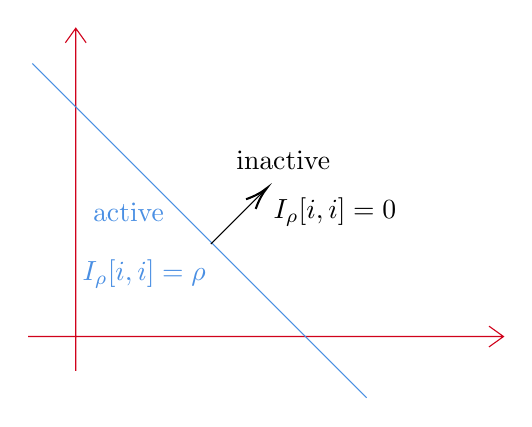
\begin{tikzpicture}[x=0.75pt,y=0.75pt,yscale=-1,xscale=1]
        \draw [color={rgb, 255:red, 208; green, 2; blue, 27 }  ,draw opacity=1 ] (50,199.54) -- (279,199.54)(72.9,51) -- (72.9,216.05) (272,194.54) -- (279,199.54) -- (272,204.54) (67.9,58) -- (72.9,51) -- (77.9,58)  ;
        \draw [color={rgb, 255:red, 74; green, 144; blue, 226 }  ,draw opacity=1 ]   (52,68) -- (213.05,229.05) ;
        \draw    (138,155) -- (163.59,129.41) ;
        \draw [shift={(165,128)}, rotate = 135] [color={rgb, 255:red, 0; green, 0; blue, 0 }  ][line width=0.75]    (10.93,-3.29) .. controls (6.95,-1.4) and (3.31,-0.3) .. (0,0) .. controls (3.31,0.3) and (6.95,1.4) .. (10.93,3.29)   ;
        \draw (149,109) node [anchor=north west][inner sep=0.75pt]   [align=left] {inactive};
        \draw (80,134) node [anchor=north west][inner sep=0.75pt]   [align=left] {\textcolor[rgb]{0.29,0.56,0.89}{active}};
        \draw (167,131.4) node [anchor=north west][inner sep=0.75pt]    {$I_{\rho }[ i,i] =0$};
        \draw (75,161.4) node [anchor=north west][inner sep=0.75pt]    {$\textcolor[rgb]{0.29,0.56,0.89}{I_{\rho }[ i,i] =\rho }$};
    \end{tikzpicture}
\end{center}

Here is a demo of how I put the AL into a quadratic form that makes taking derivatives easy (Since we don't care about constant terms, we can ignore them):

\begin{gather*}
    L_{\rho }( x,\lambda ,\mu ,\rho ) =\underbrace{\frac{1}{2} x^{T} Qx+q^{T} x+\lambda ^{T}( Ax-b) +\mu ^{T}( Gc-h)}_{\text{\ding{172}}}\\
    \underbrace{+\frac{1}{2} \rho ( Ax-b)^{T}( Ax-b)}_{\text{\ding{173}}}\\
    \underbrace{+\frac{1}{2}( Gx-h)^{T} I_{\rho }( Gx-h)}_{\text{\ding{174}}}\\
    \begin{matrix}
    \text{\ding{172}} & \frac{1}{2} x^{T} Qx+\left( q+A^{T} \lambda +G^{T} \mu \right) x\\
    \text{\ding{173}} & \frac{1}{2} x^{T}\left( \rho A^{T} A\right) x+\left( -\rho A^{T} b\right)^{T} x\\
    \text{\ding{174}} & \frac{1}{2} x^{T}\left( G^{T} I_{\rho } G\right) x+\left( -G^{T} I_{\rho } h\right)^{T} x
    \end{matrix}\\
    L_{\rho }( x,\lambda ,\mu ,\rho ) =\frac{1}{2} x^{T}\left( Q+\rho A^{T} A+G^{T} I_{\rho } G\right) x+\left( q+A^{T} \lambda +G^{T} \mu -\rho A^{T} b-G^{T} I_{\rho } h\right)^{T} x\\
    \nabla _{x} L_{\rho } =\left( Q+\rho A^{T} A+G^{T} I_{\rho } G\right) x+q+A^{T} \lambda +G^{T} \mu -\rho A^{T} b-G^{T} I_{\rho } h\\
    =Qx+q+A^{T}( \lambda +\rho ( Ax-b)) +G^{T}( \mu +I_{\rho }( Gx-h))\\
    \nabla _{x}^{2} L_{\rho } =Q+\rho A^{T} A+G^{T} I_{\rho } G
\end{gather*}

Here is the QPAL algorithm:
\begin{algorithmic}[1]
    \STATE Initialization: $x=0,\lambda=0,\mu=0,\rho=1,\phi=10$
    \WHILE {i<max\_iteration}
      \STATE Solve $x=\min_x L_\rho(x,\lambda,\mu,\rho)$. We use Newton's method to solve this unconstrained minimization of the AL w.r.t. $x$. NOTE: you can treat $I_\rho$ as constant when taking derivatives of the AL, but make sure you update $I_\rho$ every time you update $x$. Don't use line search or merit function.
      \STATE Update duals: $\lambda=\lambda+\rho(Ax-b),\mu=\max(0,\mu+\rho(Gx-h))$.
      \STATE Update $\rho=\rho\phi$.
      \STATE Check convergence: $\Vert Ax-b \Vert_\infty$ and $\max(0, \max(Gx-h))$ or check KKT conditions. You can compute constraint violations for equality with \textit{norm(Ax-b,Inf)} in Julia, and inequality with \textit{max(0,maximum(Gx-h))} in Julia. The max of these should be below some tolerance specified in the function. Alternatively, you can use the full KKT conditions as termination criteria.
    \ENDWHILE
\end{algorithmic}
\section{Exercise 1}